
\documentclass[a4paper,10pt]{article}
% This line indicates the type of the document betwin {}: here it is a scientific article.
% Options betwin [] are not mandatory, but precise here:
% - a4paper: printing paper format
% - 10pt: size of the characters

\usepackage{graphicx}
% This package allows to include images
\usepackage{titling}
% This package allows to have a subtitle 
\usepackage{listings}
% this package is used to write code samples.
\usepackage{url}
\usepackage{amsmath}
\usepackage{amsfonts}
\usepackage{amssymb}

\lstset{%
  basicstyle=\scriptsize\sffamily,%
  commentstyle=\footnotesize\ttfamily,%
  frameround=trBL,
  frame=single,
  breaklines=true,
  showstringspaces=false,
  numbers=left,
  numberstyle=\tiny,
  numbersep=10pt,
  keywordstyle=\bf
}
\newcommand{\subtitle}[1]{%
  \posttitle{%
    \par\end{center}
    \begin{center}\large#1\end{center}
    \vskip0.5em}%
}



%%%%%%%%%%%%%%%%%%%%%%%%%%%%%%%%%%%%%%%%%%%%%%%%%%%%
% Raport Headers:
%%%%%%%%%%%%%%%%%%%%%%%%%%%%%%%%%%%%%%%%%%%%%%%%%%%%
\title{Image and signal processing: Computer exercise 2}
\subtitle{CE02G02T05}
\author{SID-LAKHDAR Riyane}
\date{08/10/2015}

\begin{document}
% Beginning serious stuff. 


\maketitle
% Actually prints title / subtitle / authors and dat into the document


%%%%%%%%%%%%%%%%%%%%%%%%%%%%%%%%%%%%%%%%%%%%%%%%%%%%
% Abstract
%%%%%%%%%%%%%%%%%%%%%%%%%%%%%%%%%%%%%%%%%%%%%%%%%%%%
\begin{abstract}
  This report summarize, explains and refers to the answers we have designed for the second \"Image and Signal Processing\" computer exercise.\newline 
  The topic's questions that we are dealing with are not explicitly mentioned.  However the order of this questions have been kept to build this report.
\end{abstract}

%%%%%%%%%%%%%%%%%%%%%%%%%%%%%%%%%%%%%%%%%%%%%%%%%%%%
% Introduction
%%%%%%%%%%%%%%%%%%%%%%%%%%%%%%%%%%%%%%%%%%%%%%%%%%%%
\section{Introduction}
The aim of the current computer exercise is to have a first experimental approach with two mathematical operator often used in signal processing: the finite impulse response filter and the one dimension convolution.\newline
In this report, we will see through some specific examples the effect of this operators on some given input signals.   
All this study will try to answer, within specific conditions, to a major issue in signal processing: how to transform an input signal in a signal with the same global behavior excluding its useless or harmful feature (such as the noise or wrong samples).\newline
To make this report more readable, this report design tries to respect the convention carried on the given rapport examples.  Thus, the two main sections of this rapport:
  \begin{itemize}
   \item Material \& Methods: In this section, we described the theoretical methods used to answer to our different questions.  We provide the expected algorithms, them main principles or them python implementation.
   \item Experiments: In this section, we give the experimental results of our experiences.  We try to explain them, and see whether they are consistent with the theoretical expectations or not.
  \end{itemize}

\section{Material \& Methods}
    \subsection{Linear and finite impulse response filters}
	\subsubsection{Finite impulse response filters}
	In signal processing, a finite impulse response (FIR) filter is a system where the non-zero part of the impulse response is finite in extent.[ref: http://www.eas.uccs.edu/].\newline
	Thanks to this property, given a FIR S, for each input signal x, the number of different values n where s(x)[n] is different from zero is finite (however x is an infinite length signal).
	Thus, the convolution of filtered signals may be written as:
	\begin{equation*}
	\begin{aligned}
	    (S(x_{1}) * S(x_{2}))[n]
	        &= \sum_{m=-\infty}^{+\infty} (S(x_{1})[m] * S(x_{2})[n-m]) \\
	        &= \sum_{m \in N} (S(x_{1})[m] * S(x_{2})[n-m]) \\
	\end{aligned}
	\end{equation*}
	Where N is a finite set of values where
	\begin{equation} \forall v \in N, S(x_{1})[v] \ne 0 \mbox{ and } S(x_{2})[v] \ne 0 \mbox{ and} \end{equation}
	\begin{equation} \forall v \notin N, S(x_{1})[v] = S(x_{2})[v] = 0 \end{equation}
	To summarize, a finite impulse response filter allows to compute the convolution of infinite length signals (which are not equal to zero from a given point) as a finite sum.\newline
	In the first part of the report, we will consider the following finite impulse response system:
	\begin{equation} S(x)[n] = y[n] = 0.5 * x[n] + 0.95 * y[n] \end{equation}


	\subsubsection{Ensure the linearity of our system}
	Let consider y0 a fixed value, and let suppose that each one of the filter input signal x respects the condition x[0] = y0.\newline
	To prove that, under this condition, our system is linear, we need to prove that the system is linear, we need to prove that it verifies the homogeneity and the additive properties:
	\begin{itemize}
	    \item
		Let x a given signal. and a a fixed value.\newline
		\begin{equation*}
		\begin{aligned}
		    \forall n \in  \mathbb{N}, S(a x)[n]
		    &= 0.05 (a x[n]) + 0.95 (a y[n-1])\\
		    &= a (0.05 x[n] + 0.95 y[n-1]) \mbox{ //associativity and the comutativity of the multiplication)}\\
		    &= a S(x)[n]\\
		\end{aligned}
		\end{equation*}
		Thus, S is homogeneous
	    \item
		Let A(n) the property: S respects the additivity condition for each input rank smaller or equal n.  Let's prove A by induction:
		\begin{equation} \forall \mbox{ input signals } x_{1}, x_{2}, \end{equation}

		\begin{equation*}
		\begin{aligned}
		    S(x_{1} + x_{2})[1]
		    &= 0.05 (x_{1}+x_{2})[1] + 0.95 S(x_{1}+x_{2})[0]\\
		    &= 0.05 (x_{1}+x_{2})[1] + 0.95 S(2 y_{0})\\
		    &= 0.05 (x_{1}+x_{2})[1] + 2*0.95 S(y_{0})\mbox{ // Because S is homogenious}\\
		    &= 0.05 (x_{1})[1] + 0.95 S(y_{0}) + 0.05 (x_{2})[1] + 0.95 S(y_{0})\mbox{// distributivity of the sum}\\
		    &= S(x_{1})[1] + S(x_{2})[1]\\
		    \mbox{Thus, A(1) is true}
		\end{aligned}
		\end{equation*}
		Assuming that A(n-1) is true for a fixed n, let's now prove A(n):
		\begin{equation} \forall n \in  \mathbb{N}\mbox{, and } x_{1}, x_{2}\mbox{ input signals,  }\end{equation}
		\begin{equation*}
		\begin{aligned}
		    S(x_{n} + x_{2})[n]
		    &= 0.05 (x_{1}+x_{2})[n] + 0.95 S(x_{1}+x_{2})[n-1]\\
		    &= 0.05 (x_{1})[n] + 0.05 (x_{2})[n] + 0.95 S(x_{1}+x_{2})[n-1] \mbox{ // distributivity of the sum}\\
		    &= 0.05 (x_{1})[n] + 0.05 (x_{2})[n] + 0.95 S(x_{1})[n-1] + 0.95 S(x_{2})[n-1] \mbox{ // Because A(n) is true}\\
		    &= S(x_{1})[n] + S(x_{2})[n]\\
		\end{aligned}
		\end{equation*}
		Thus, we have proved that A(n) is true.\newline
		Hence S is additive.
	\end{itemize}
	As we have proven the homogeneity and the additivity of S, we can say that assuming that x[0] is constant for each input signal x, S is linear.


	\subsubsection{First use of this filter}
	To have a practical approach of the previously defined system, we first need to define some input signals.  First of all, we have defined some basic signals in the following figure.
	\begin{lstlisting}
def signalX1(sampleSize):
    signal      = [0.5] * sampleSize
    signal[0]   = y0_linearitycondition
    for k in range(1, sampleSize):
        signal[k] = math.sin((math.pi*k)/50)
    return signal

def signalX2(sampleSize):
...

def signalX3(sampleSize):
...

\end{lstlisting}
	Finally, the next program is the representation of our filter.\newline
	\begin{lstlisting}
def singleLowPassFilter(inputSignal):
    sampleSize      = len(inputSignal)
    outputSignal    = [0.5] * sampleSize
    outputSignal[0] = y0_linearitycondition
    for k in range(1, sampleSize):
        outputSignal[k] = 0.05 * inputSignal[k] + 0.95 * inputSignal[k-1]
    return outputSignal
	\end{lstlisting}
	The experimental results of our programs and the theoretical consequences of this results on the defined filter are given in the Experiments section of this report (3.1).\newline



	\subsubsection{Add a noise signal to the filter's input signal}
	In addition to the 3 signal previously defined, we have defined the following Gaussian noise signal.
	This signal is a Gaussian function where every sample's value has been perturbed by a random bounded value.
	\begin{lstlisting}
#-----------------------------------
# Gaussian noise parameters
#-----------------------------------
gaussianAmplitude   = 5
gaussianCenter      = nbrSample/2
gaussianWidth       = 50
gaussianRandomBoud  = 0.5
random.seed(10)


def signalX4(sampleSize):
signal      = [0.5] * sampleSize
signal[0]   = y0_linearitycondition
for k in range(1, sampleSize):
    tmpNumerator    = -1* math.pow((k-gaussianCenter), 2)
    tmpdenominator  = 2 * math.pow(gaussianWidth, 2)
    signal[k] = gaussianAmplitude * math.exp(tmpNumerator / tmpdenominator)
    # add a random noise to the gaussian
    signal[k] = signal[k] + random.uniform(-gaussianRandomBoud, gaussianRandomBoud)
return signal
	\end{lstlisting}
	In the Experiments section, we will describe the influence of this specific noise shape signal on our system.

	
	
    \subsection{1D convolution}
	\subsubsection{Definition and first approach}
	The convolution is a mathematical operation on two functions, which produces a third function. It is defined as the sum of the product of the two functions after one is reversed and shifted.
	[ref: http://www.eas.uccs.edu/]\newline
	\begin{lstlisting}
# x and y are two discrete causal signals
# this returns sum of each x[l].y[k-l] for l ranging from 0 to k
def convolution_sum(x, y, k):
	temp_x = fillWithZeros(x, k+1)
	temp_y = fillWithZeros(y, k+1)
	res_sum = 0
	for l in range(0, k+1):
		res_sum += temp_x[l] * temp_y[k-l]
	return res_sum
def myConvolution1D(x, y):
   length = len(x) + len(y) - 1
   m = np.zeros(length)
   for k in range(0, length):
   	m[k] = convolution_sum(x, y, k)
   return m
   \end{lstlisting}
	\subsubsection{Instance of 1D Convolution: Moving Average Filter}
	The Moving Average Filter is a filter with the purpose of removing random noise while retaining a sharp step response. It operates by averaging a number of points from the input signal to produce each point in the output signal.\newline
	It's equations is as follows :
	\begin{equation}
    y[k] = \frac{1}{M} \sum_{p=-\frac{M-1}{2}}^{\frac{M-1}{2}} x[k+p]
\end{equation}	\newline
where x is the input signal, y the output signal and M is the odd number of points used in the moving average.

Now let us use a change of variables : k becomes k-(M-1/2)\newline
\begin{equation}
    y[k - \frac{M-1}{2}] = \frac{1}{M} \sum_{l=0}^{M-1} x[k-l] = z[k]
\end{equation}

Let h = {1/5, 1/5, 1/5, 1/5, 1/5} and M = 5.  For a given input signal x, the convolution of x and h may be written as:
\begin{equation*}
	\begin{aligned}
	    (x * h)[k]
	        &= \sum_{l=0}^{k} x[l] h[k-l] \\
	        &= x[0] h[k] + x[1] h[k-1] + ... + x[k-1] h[1] + x[k] h[0]\\
	        &= (\sum_{i=0}^{k-5} x[i]*0) + x[k-4] * \frac{1}{5} + x[k-3] * \frac{1}{5} + x[k-2] * \frac{1}{5} + x[k-1] * \frac{1}{5} + x[k] * \frac{1}{5}\\
	        &= 0 + (\sum_{l=0}^{4} x[k-l] * \frac{1}{5})\\
	        &= (\sum_{l=0}^{M-1} x[k-l] * \frac{1}{M}) \mbox{ where M = 5}\\
	        &= z[k]
	\end{aligned}
	\end{equation*}

	So z is a convolution, this means that y, which is just a time shift of z, behaves like a convolution.  Thus, we can use our "myConvolution1D" python function to compute the moving average filter : \newline
	
	
	\begin{lstlisting}
	def getMAF_FromConvolution(z, M):
	    shift = int((M-1)/2)
	    length = len(z) - shift
	    y = np.zeros(len(z))
	    for k in range(0, length):
		    y[k] = z[k+shift]
	    return y
	\end{lstlisting}

\section{Experiments}
    \subsection{Linear and finite impulse response filters}
	\subsubsection{Input signals description}
	In the section (2.1.3), we have experimentally defined the 3 signals given by the following expression:
	\begin{equation}
	\begin{aligned}
	    x_1 &= sin\left(\frac{2 \pi}{100}\right)\\
	    x_2 &= 4e^{-\frac{(n-150)^2}{300}} - e^{-\frac{(n-150)^2}{2500}}\\
	    x_3 &= 
		\begin{cases}
			1 & \textbf{if } 240 < n < 300 \\
		-2 & \textbf{if } 299 < n < 380 \\
		0 & \textbf{otherwise}\\
		\end{cases}\\
	x_4 &= \textbf{Gaussian Noise}
	\end{aligned}
	\end{equation}\label{signalsFormula}
	All the filter's qualitative analysis in this section will refer to this functions.

            
	
	\subsubsection{Filter response to basic signals}
	Once we have defined our signals, and the filter's algorithm, we can, experimentally, analyze the behaviour of our filter.  In this section, we will only analyze the behaviour of the filter on the basic signals previously defined.  Thanks to the Figure: \ref{Signal_image}, we can notice that:
	\begin{figure}[!htb]\centering
	  \begin{minipage}{0.45\textwidth} \frame{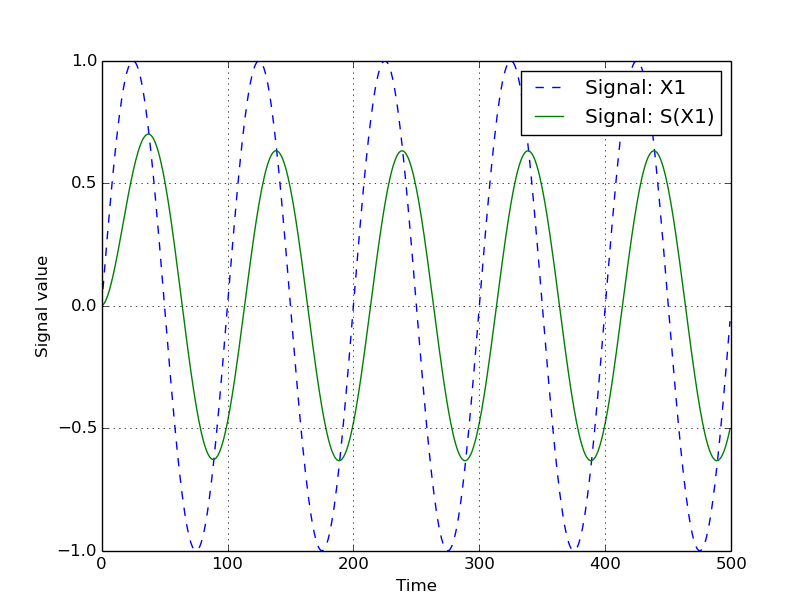
\includegraphics[width=\linewidth]{question1_6_X1_S(X1).png}} \end{minipage}
	  \begin{minipage}{0.45\textwidth} \frame{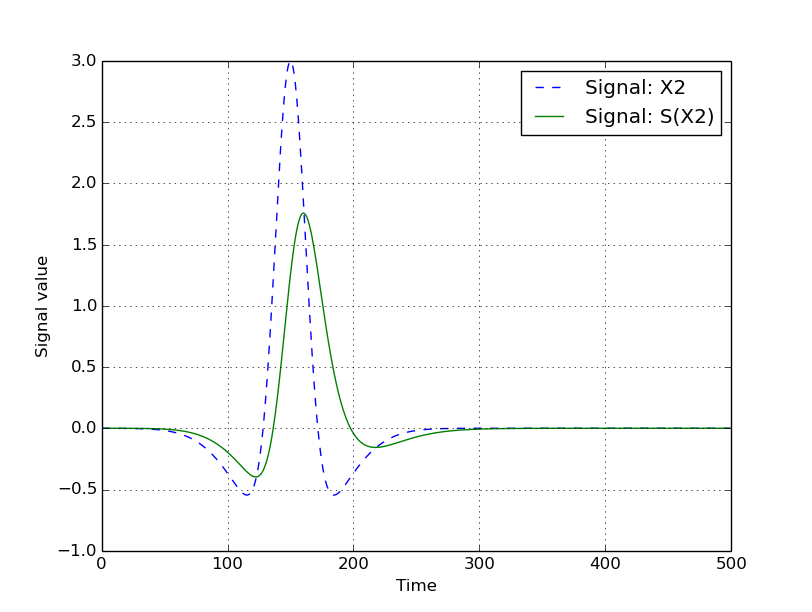
\includegraphics[width=\linewidth]{question1_6_X2_S(X2).png}} \end{minipage}
	  \begin{minipage}{0.45\textwidth} \frame{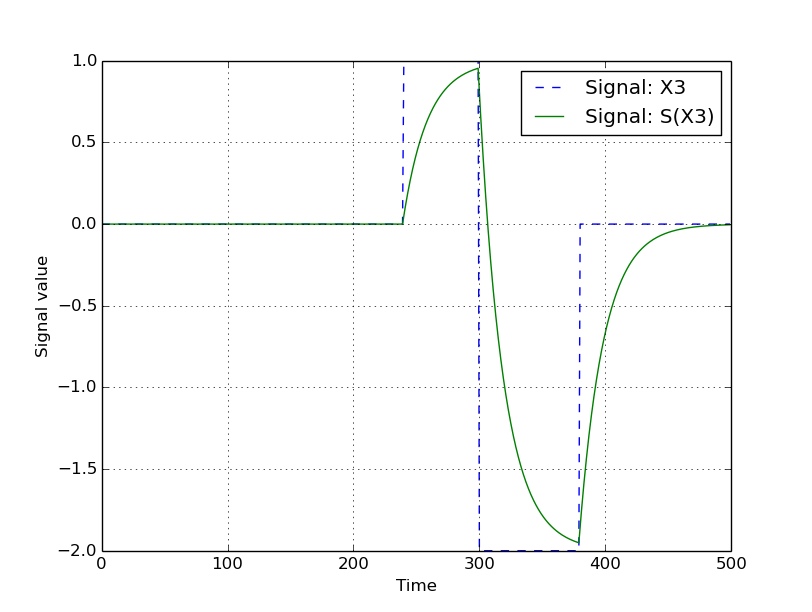
\includegraphics[width=\linewidth]{question1_6_X3_S(X3).png}} \end{minipage}
	  \begin{minipage}{0.45\textwidth} \frame{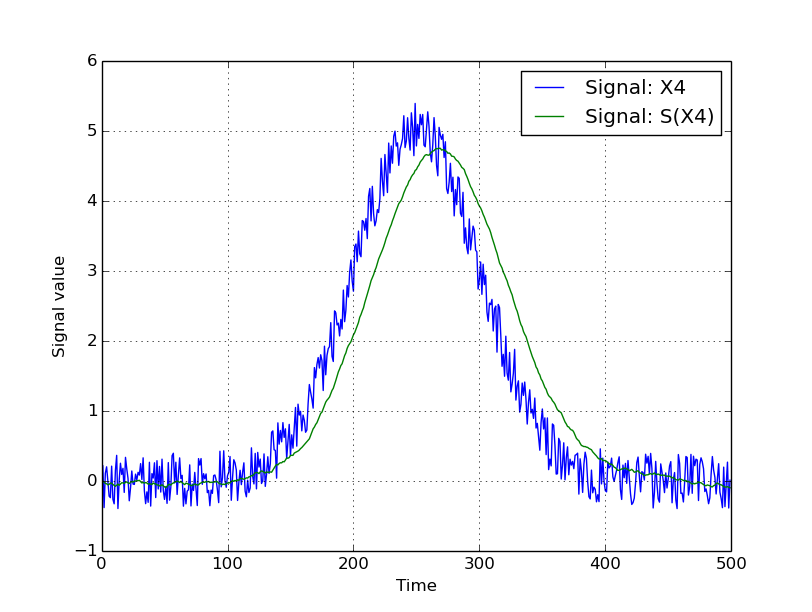
\includegraphics[width=\linewidth]{question1_6_X4_S(X4).png}} \end{minipage}
	  \caption{Input signals and them image through the filter}
	  \label{Signal_image}
	\end{figure}
	\begin{itemize}
	 \item The amplitude of the image is always smaller than the amplitude of the input signal (the filtered signal may be softened).
	 \item The input signal may be shifted compared to its image through the filter
	 \item The signal and its image have the same evolution: same sequence of global increasing and decreasing. For sure, this statement does not consider the noisy signals.
	\end{itemize}
	Thus, the images we computed have many likeness with them input signals, which makes this filter intresting for signal processing purposes.   
	However, this images are never the exact copy of the input signals.  Thus, the filter creates a loss of data.



	\subsubsection{Experimental proof of the filter's linearity}
	An other usefulness of this experimental representation is to confirm theoretical results:\newline
	For instance, the figure \ref{filtere of sum} and \ref{sum of filtere}, we have ploted the signal (S(x1) + S(x2) + S(x3)) on the left, and the signal S(x1 + x2 + x3) on the right.
	\begin{figure}[!htb]\centering
	  \begin{minipage}{0.45\textwidth}
	  \frame{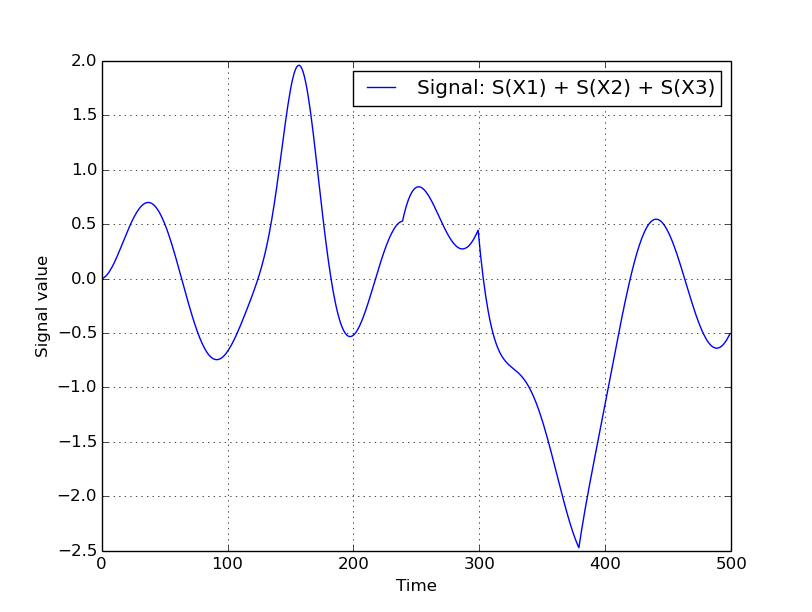
\includegraphics[width=\linewidth]{question1_6_signalS(X1)+S(X2)+S(X3).png}}
	    \caption{S(X1)+S(X2)+S(X3)}\label{sum of filtere}
	  \end{minipage}
	  \begin{minipage}{0.45\textwidth}
	  \frame{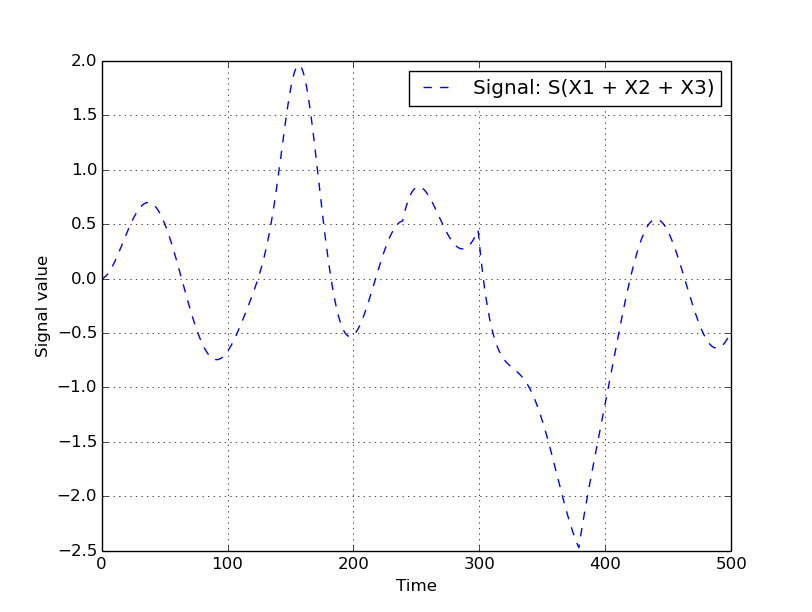
\includegraphics[width=\linewidth]{question1_6_signalS(X1+X2+X3).png}}
	    \caption{S(X1+X2+X3)}\label{filtere of sum}
	  \end{minipage}
	\end{figure}
	As you may have noticed, the two signals have the exact same values, on them whole definition domain.  Which confirmes the additivitycaracter of the filter (proved in the section 2.1.2).\newline
	The homogeneity of the filter has been experimentally confirmed using the same kind of trick: for a given signal x, we have compared the plots of the function  S(ax) and aS(x), for sevral fixed values of a.\newline

	
	
	\subsubsection{Adding a noise}
	Let's now consider the gaussian noise x4, which python representation has been given in the section 2.1.4, and which graphical representation is given Figure: \ref{signal X4}.  
	Thanks to this program, we can create a signal XNoise = (x1+x2+x3+x4) and compute its image through our filter (figure \ref{xNoise and S(xNoise)}).\newline
	\begin{figure}[!htb]\centering
	  \begin{minipage}{0.45\textwidth}
	  \frame{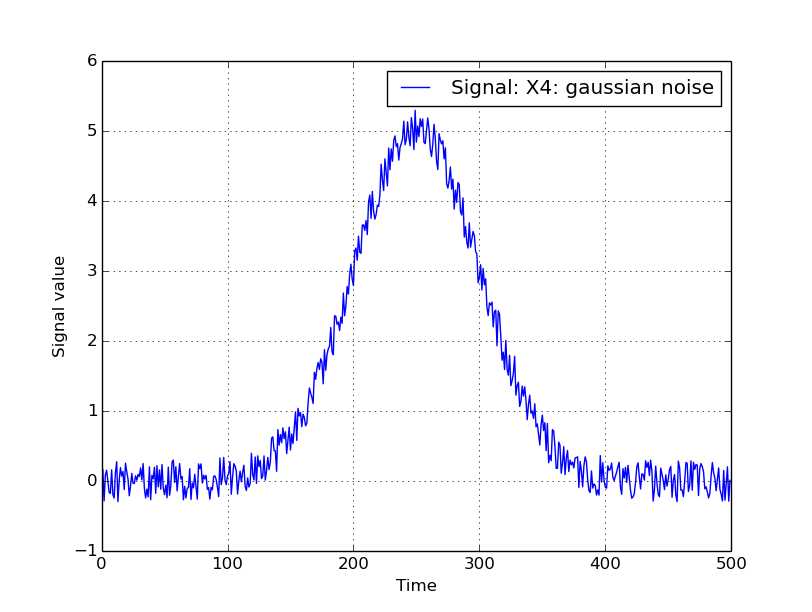
\includegraphics[width=\linewidth]{question1_10_signal_X4.png}}
	    \caption{Signal X4: gaussian noise }\label{signal X4}
	  \end{minipage}
	  \begin{minipage}{0.45\textwidth}
	  \frame{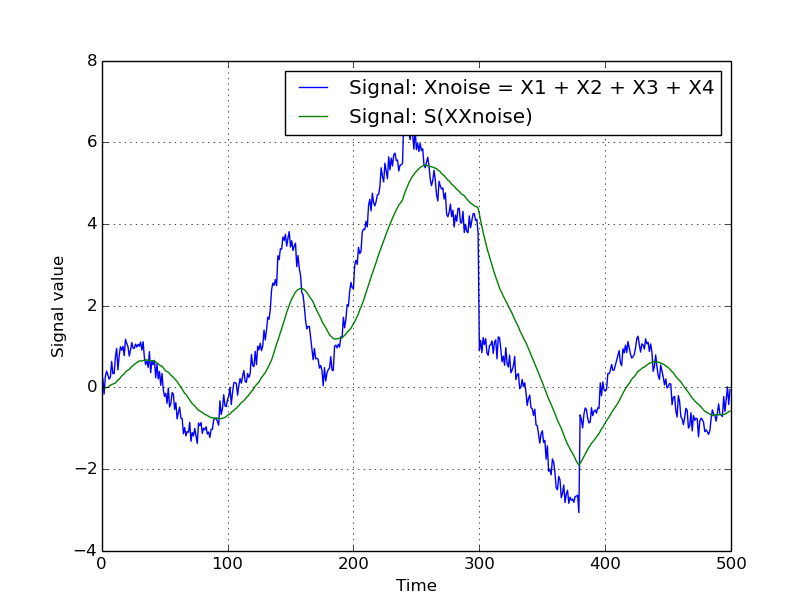
\includegraphics[width=\linewidth]{question1_10_signalXNoise+filter.png}}
	    \caption{Signal xNoise and its image through the filter}\label{xNoise and S(xNoise)}
	  \end{minipage}
	\end{figure}
	As we can see on the figure \ref{xNoise and S(xNoise)}, the noisy signal and its image through the filter have the same behaviour (global variation excluding noise variation on the input).  
	However, thanks to the filter, the noise has been subdued.   Thus, this filter allows (on this gaussian noise example) to create an output signal with the same assymptotic and global behaviour as the input.  The input signal is purified.
	
	
    \subsection{1D convolution}
	\subsubsection{Definition and first approach}
	Here we used the convolution algorithm we wrote to convolve the input signal  x={1;0;2;3;2;1;−1;−2;−1;0;2;3;3;2;1;1} with the impulse response: h={2;2;−1;−1;3}\newline
	These different signals are ploted in the figure \ref{1Dconvolution}:\newline
	\begin{figure}[!htb]\centering
	\begin{minipage}{0.45\textwidth\centering}
	  \frame{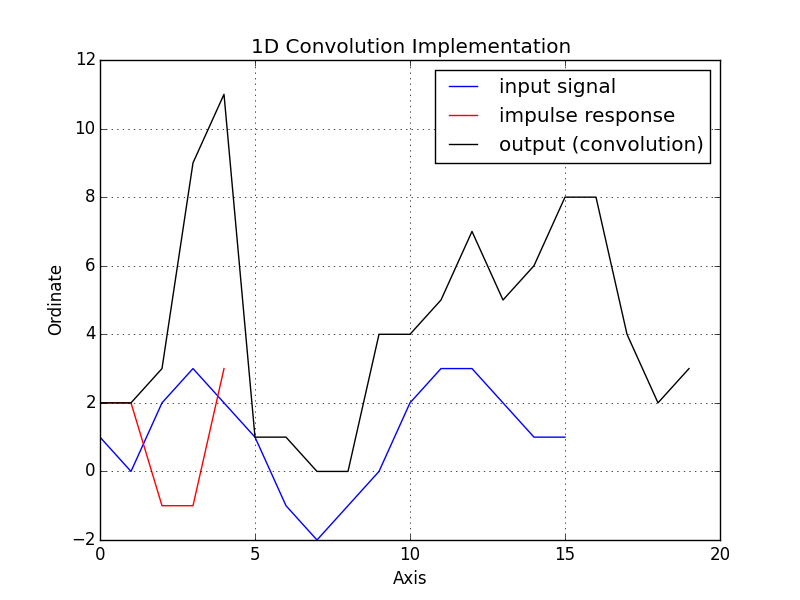
\includegraphics[width=\linewidth]{question2_2_basic_convolution.png}}
	  \caption{representation of the 1D convolution of the signals x and h}
	  \label{1Dconvolution}
	  \end{minipage}
	  \end{figure}
	  
	\subsubsection{Instance of 1D Convolution: Moving Average Filter}
	Now we apply the Moving Average Filter to our previous signal Xnoise (with M = 5, and M = 51) : figure: \ref{Moving average filter}
	\begin{figure}[!htb]\centering
	\begin{minipage}{0.45\textwidth}
	\frame{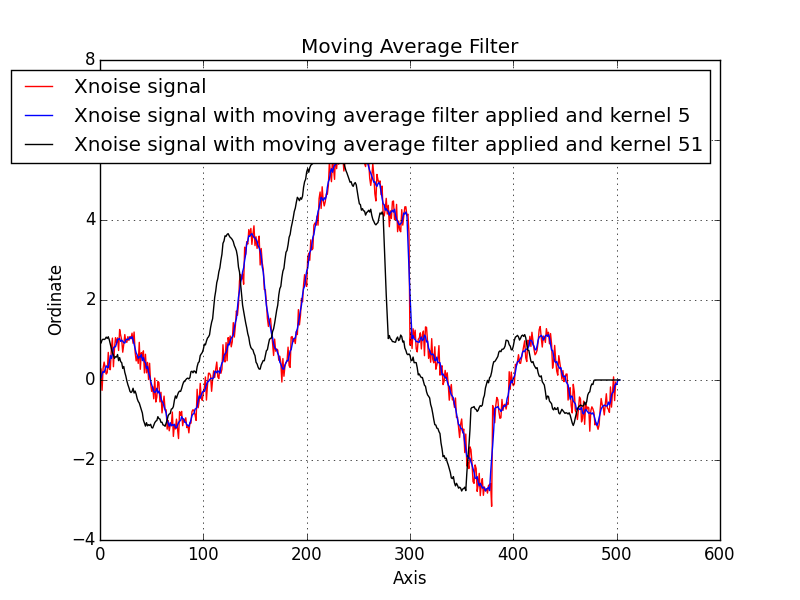
\includegraphics[width=\linewidth]{question2_6_moving_average_filter_51.png}}
	\end{minipage}
	\caption{Moving average filter}
	\label{Moving average filter}
	\end{figure}

	Now we try the same thing but with M = 51.
	We notice that 51 shifts the signal too much, it is out of sync with Xnoise.
	The Moving Average Filter is effective at filtering with minimal loss of data, however it keeps a little bit of the noise, and the number of points used in the moving average must be chosen carefully or the output signal will be shifted too far.	

\end{document}
